% % % % % % % % % % % % % % % % % Preamble for notes % % % % % % % % % % % % % % % % % % % % % % % %
\documentclass[12pt,oneside,a4paper]{article}


% % % % % Sprogpakker og Layout % % % % % % % % %
\usepackage[left=2.5cm,top=2.0cm,bottom=1.5cm, right=3.0cm]{geometry}
\usepackage{ulem}
\usepackage[danish,english]{babel}
\usepackage[utf8]{inputenc}
\linespread{1.3}       % simulerer Word 1.5 line spacing

% % % % % % % % % % Øvrige vigtige pakker % % % % %
\usepackage{graphics}
\usepackage{amsmath}
\usepackage{amssymb}
\usepackage{url}
\usepackage{cancel}
\usepackage{booktabs}
\usepackage{pdfpages}
\usepackage{mathpazo}
\usepackage[section]{placeins}
\usepackage{caption}
\usepackage{wrapfig}
\usepackage{tocloft}
\usepackage{subfig}
\usepackage{fancyhdr}
%Muliggør 'flere figurer i én' Eksempel på anvendelse (indenfor figure-environment):
% \subfloat[undercaption 1]{\label{label 1}\includegraphics[bredde 1]{billede 1}}
% \subfloat[undercaption 2]{\label{label 2}\includegraphics[bredde 2]{billede 2}}
% \caption{overordnetcaption}
% \label{overordnet label}
\usepackage{lscape}
%Omdanner en del af dokumentet til landscape. Angives med \begin{landscape}
\usepackage{framed}
%Sætter en ramme om et område begrænset af \begin{framed} og \end{framed}.
%Allows footnotes
\usepackage{footnote}
\setlength{\parindent}{0cm}
\setlength{\parskip}{0.3cm}
% % % % % % COMMANDS % % % % % % % %

\begin{document}

\selectlanguage{english}
% % % % % % % % % % % % % % % % % % % % % % Forside % % % % % % % % % % % % % % % % % % % % % % % % %
\pagenumbering{roman}

\begin{center}
{\textsc {\LARGE \bf{Københavns Universitet \\[0.3cm]  Bachelorstudiet i fysik}}}\\[1.5cm]
{\textsc {\Large \bf Førsteårsprojekt 2017}}\\[0.8cm]
{\Large Projekt nummer: 2017-06}\\[1cm]

\rule{15cm}{0.01cm}\\[1cm]
{\LARGE\bf  Bouncing ball}\\ [0.5cm]
\rule{15cm}{0.01cm}\\[1cm]
\end{center}

\vfill
{\large Forfattere:}\\
{\large \hspace*{1cm} \makebox[6cm][l]{Andreas M. Faber}  \hspace{1cm} KU- ID: \makebox[2cm][l]{QZJ517} \\
{\large \hspace*{1cm} \makebox[6cm][l]{Benjamin T. Søgaard}   \hspace{1cm} KU- ID: \makebox[2cm][l]{MGX877} \\
{\large \hspace*{1cm} \makebox[6cm][l]{Joachim J. Kønigslieb}   \hspace{1cm} KU- ID: \makebox[2cm][l]{GWC666} \\

{\large Vejledere:}\\
{\large \hspace*{1cm} \makebox[6cm][l]{Jörg Helge Müller}  \hspace{1cm} Email: \makebox[2cm][l]{muller@nbi.ku.dk} \\

\vfill

{\large Rapporten omfatter {\bf 1} siders hovedtekst og {\bf 1} siders appendix.}

{\large Rapporten er indsendt som en pdf-fil den 17 marts 2017. }

\normalsize


% % % % % % % % % % % % % % % % % % % % % % Abstract  og Indholdsfortegnelse % % % % % % % % % % % % % % % % 
\newpage
\begin{abstract}
Kort resumé, gerne på både dansk og engelsk.
\end{abstract}

\newpage

\tableofcontents


% % % % % % % % % % % % % % % % % % % % % % Indhold % % % % % % % % % % % % % % % % % % % % % % % % %
\newpage
\pagenumbering{arabic}
\section{Introduction to chaos}

asdfagaffhåijpsfgh

\section{The experiment}

\section{Model of the system}
We will model our experiment as a 1-dimensional system that is we will not account for sideways movements. On figure \ref{bounces} two consecutive bounces can be seen where the later is bigger due to the plate is moving upwards at the time of impact.
\begin{figure}[h]
	\centering
	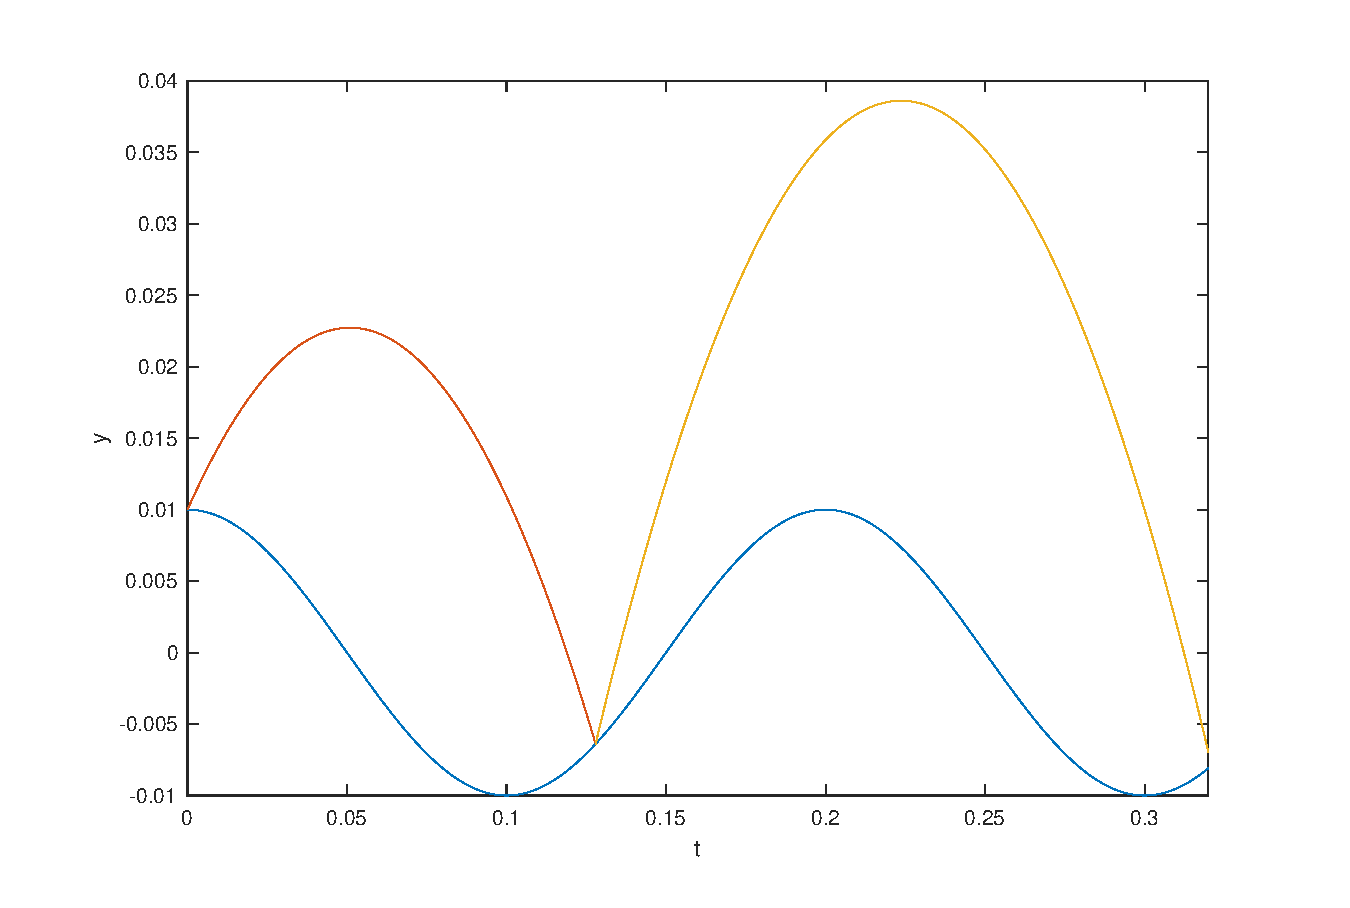
\includegraphics[width=0.6\textwidth]{Figures/bounceplot.eps}
	\caption{Plot of two bounces on the vibrating plate}
	\label{bounces}
\end{figure}
The $k$th bounce can be completely described by the time $t_k$ it left the plate and the velocity $v_k$ at that instance. Time and phases $\phi_k$ can be used interchangeably through the relation ship $\phi=2\pi f t$.

To describe the system during a specific bounce we denote the distance of the ball above the plates rest position $y_b(t)$. Similarly we define $y_p(t)$ as the displacement of the vibrating  plate from it equilibrium. For a given frequency $f$, phase shift $\phi$ and amplitude $A$ the equation of motion for the plate is
\begin{equation}
	y_p(t)= A \sin(2\pi f t+ \phi)
	\label{platey}
\end{equation}
In air the ball is essentially a body in free fall, and since it is quite small and dense, the air resistance can be ignored. Thus the equation of motion for the ball $y_b(t)$ for a specific initial condition $v_i$, $y_i$ at time $t_i$ is simply 
\begin{equation}
	y_b(t) = -\frac{g}{2}(t-t_i)^2+v_i(t-t_i)+y_i
\end{equation}
To model the impact between the ball and the plate we use a constant coefficient of restitution $C_r$ although more complex models have been suggested. For a plate at rest the velocity after the impact is proportional to the velocity before by $C_r$ such that $v_f=C_rv_i$. For a moving plate we simplify transform into the coordinate system where the plate is at rest and then transform back. Deriving equation (\ref{platey}) with respect to $t$ yields the velocity of the plate, which gives the following relationship between $v_{in}$ and $v_{out}$
\begin{equation}
	v_{out} = C_r(v_{in}-v_b)+v_b= 
\end{equation}

% % % % % % % % % % % % % % % % % % % % % % Appendix % % % % % % % % % % % % % % % % % % % % % % % % %
\newpage
\appendix
\section{Appendix}
Her er appendix. Husk at appendix ikke indgår i bedømmelsen af rapporten. Det kan bruges til supplerende udregninger, figurer eller programkode, som ikke er nødvendig for forståelsen af rapportens indhold.



\end{document}
